\section{Durchführung}
\label{sec:Durchführung}
\subsection{Aufbau}
Um die Zielsetzung des Versuchs zu erreichen, werden die 3 in \autoref{fig:aufbaua}, \autoref{fig:aufbaub} und \autoref{fig:aufbauc} zu sehenden Schaltungen aufgebaut.
\begin{figure}[H]
    \centering
    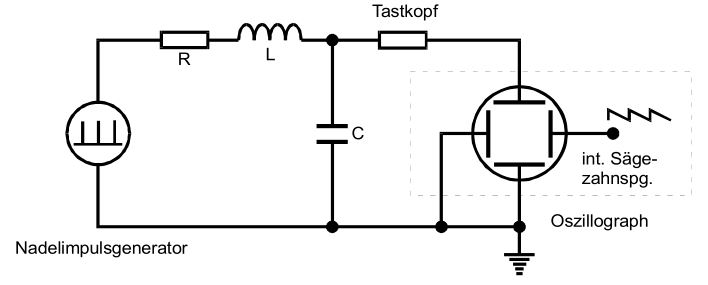
\includegraphics[width=\textwidth]{bilder/aufbaua.JPG}
    \caption{Schaltung zur Messung der Zeitabhängigkeit der Amplitude der gedämpften Schwingung. \cite{sample}}
    \label{fig:aufbaua}
  \end{figure}
\noindent

\begin{figure}[H]
    \centering
    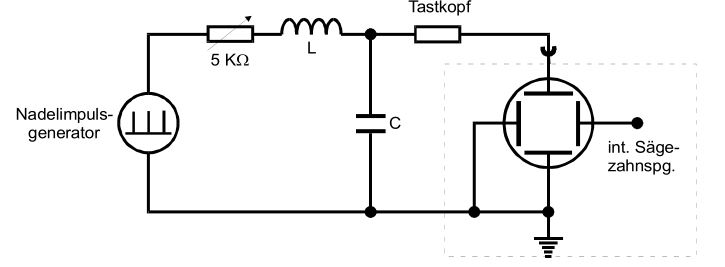
\includegraphics[width=\textwidth]{bilder/aufbaub.JPG}
    \caption{Schaltung zur Messung des aperiodischen Grenzwiderstandes $R_{\text{ap}}$. \cite{sample}}
    \label{fig:aufbaub}
  \end{figure}
\noindent

\begin{figure}[H]
    \centering
    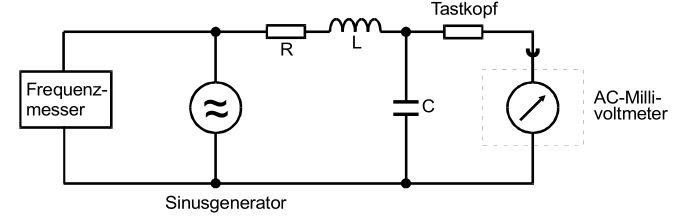
\includegraphics[width=\textwidth]{bilder/aufbauc.JPG}
    \caption{Schaltung zur Messung der Frequenzabhängigkeit der Kondensatorspannung eines RLC-Kreises. \cite{sample}}
    \label{fig:aufbauc}
  \end{figure}
\noindent
Für die Realisierung der 3 Messschaltungen wird die in \autoref{fig:schaltung} abgebildete Apparatur genutzt.
\begin{figure}[H]
    \centering
    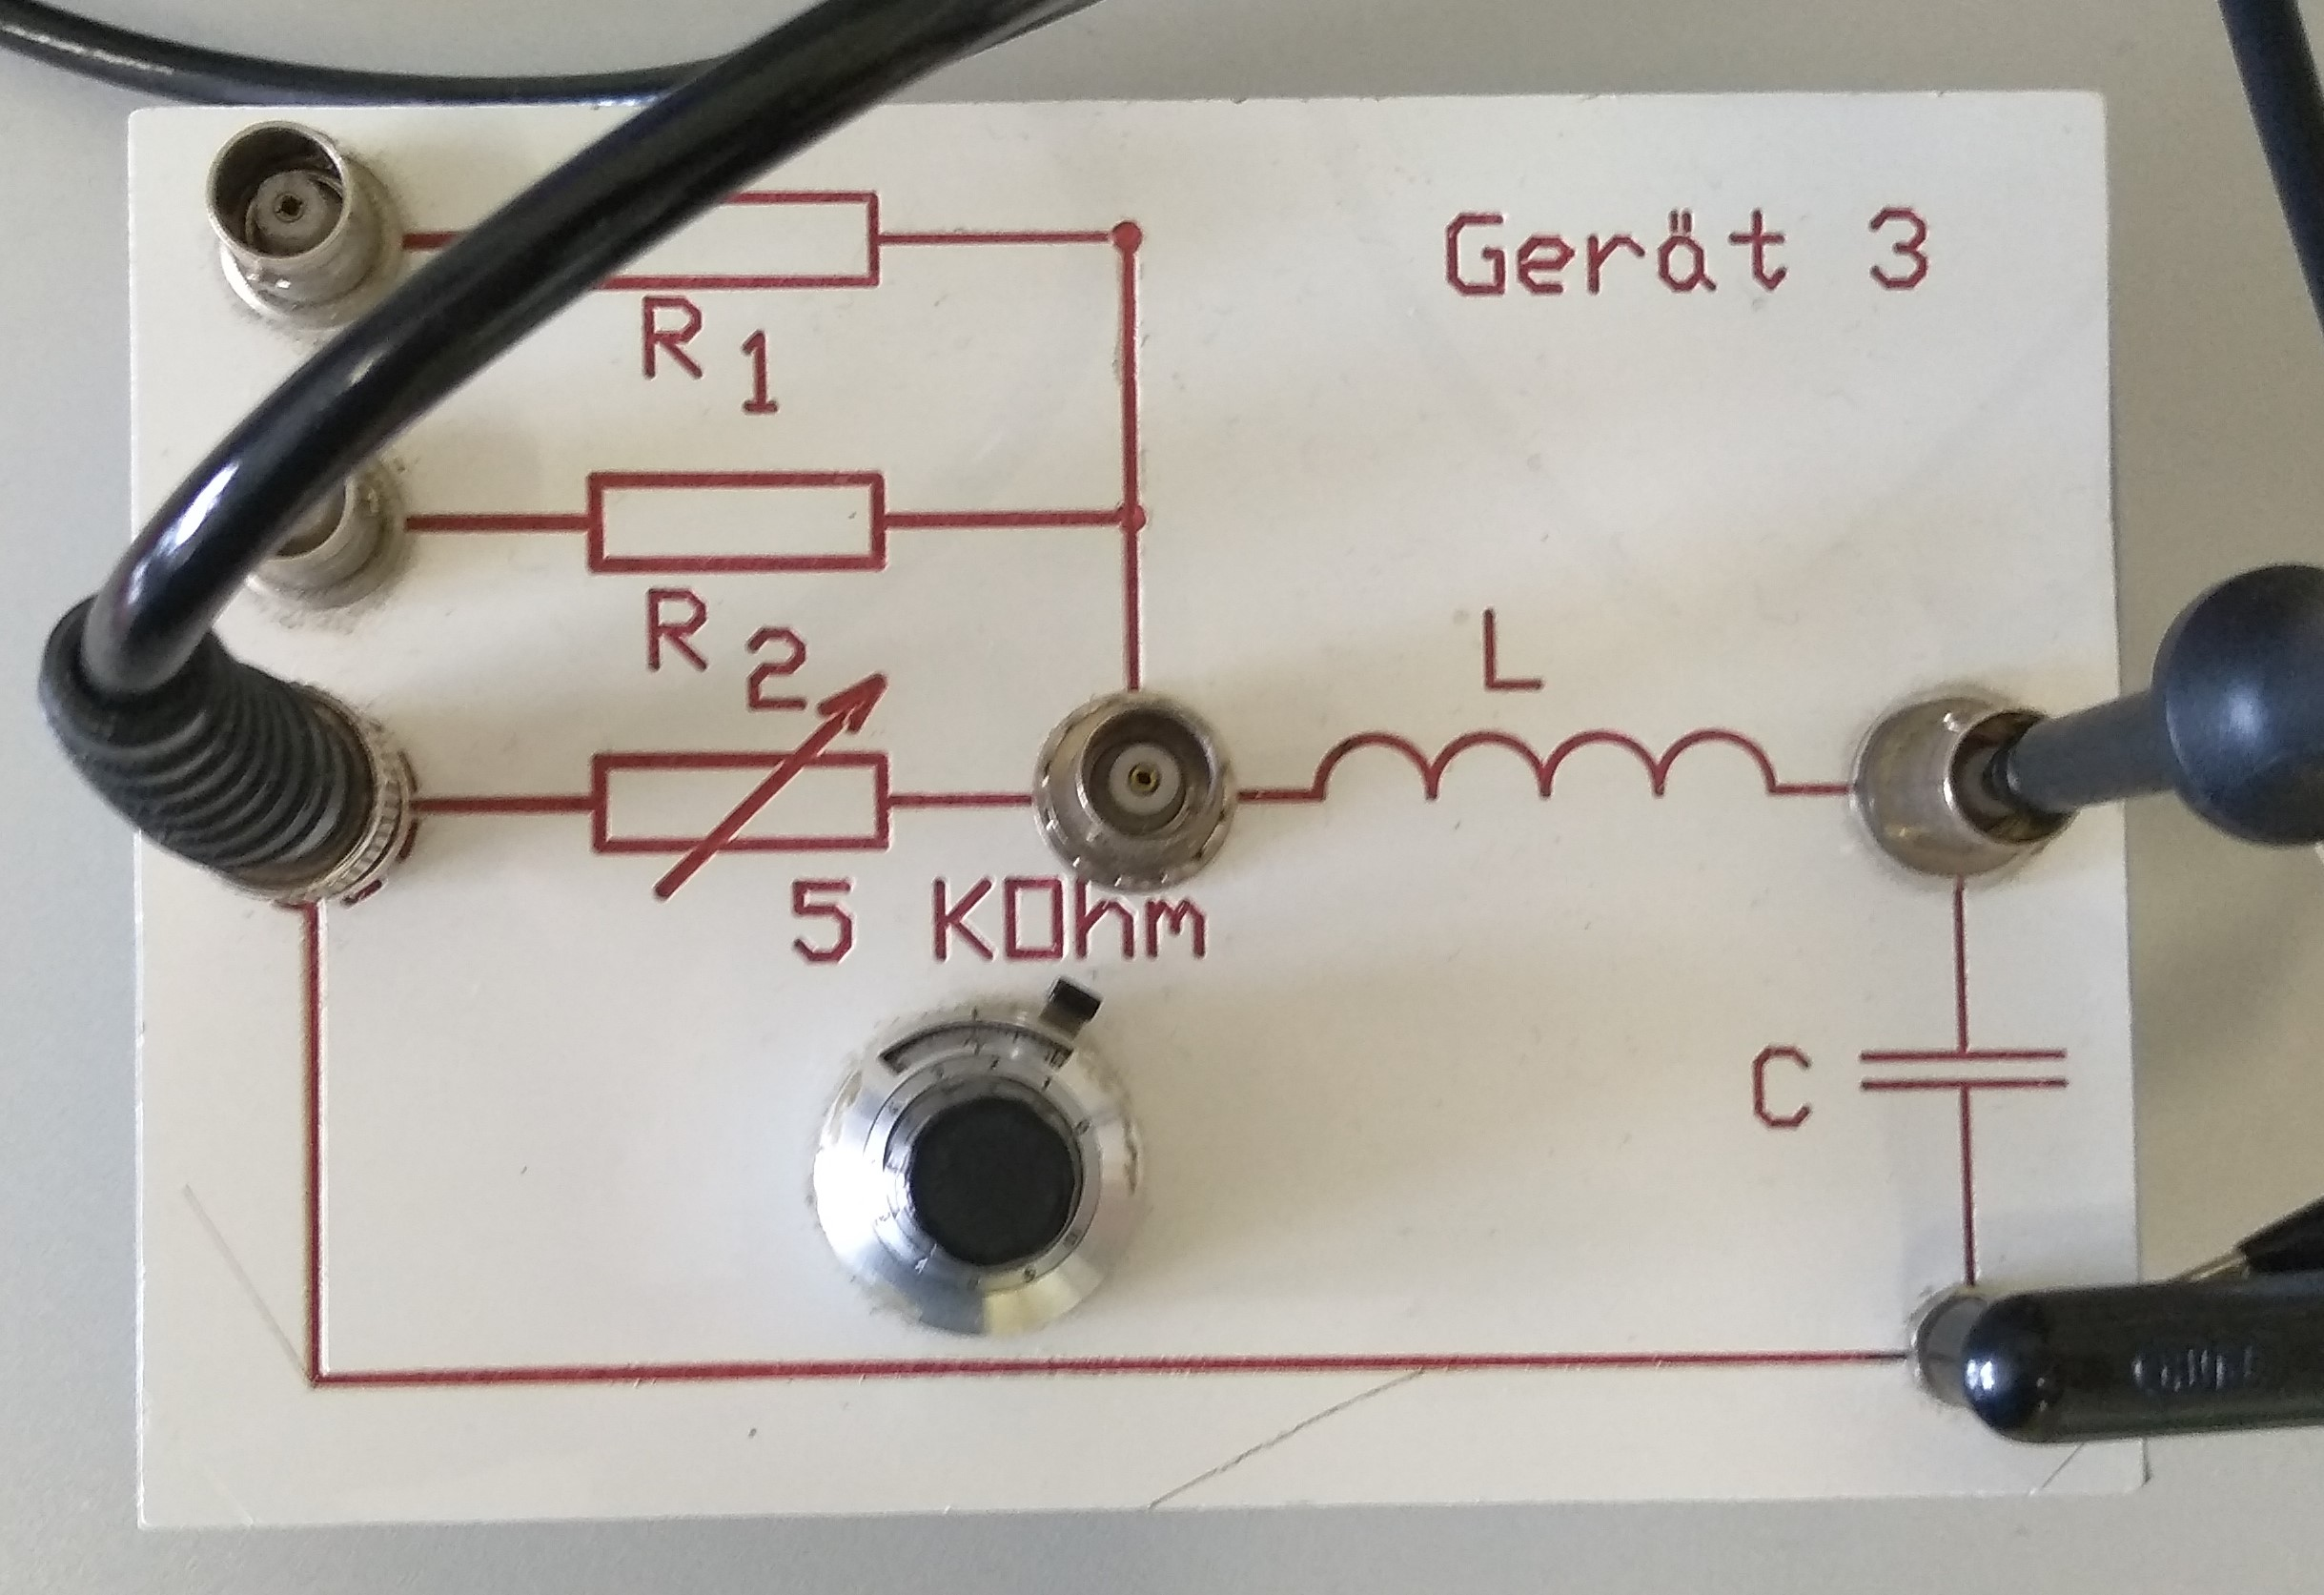
\includegraphics[width=\textwidth]{bilder/schaltung.jpg}
    \caption{Apparatur zur Realisierung der Messschaltungen.}
    \label{fig:schaltung}
  \end{figure}
\noindent
Diese Apparatur besitzt neben den festen Widerständen $R_1$ und $R_2$ einen regelbaren Widerstand. Als Werte für die weiteren Bauelemente sind $C=(5\pm0,02) nF$ und $L=(3,5\pm0,01) mH$ angegeben.
\subsection{Vorgehensweise}
Zur Bestimmung der Zeitabhängigkeit der Spannungsamplitude wird die Schaltung aus \autoref{fig:aufbaua} genutzt und durch die Apparatur aus \autoref{fig:schaltung} realisiert. So werden am Oszilloskop möglichst viele Messwerte für die Spannungsamplitude in Abhängigkeit von der Zeit abgelesen. \newline
Für die Bestimmung des Widerstands $R_{\text{ap}}$, bei dem der aperiodische Grenzfall auftritt, wird mit der Schaltapparatur die Schaltung aus \autoref{fig:aufbaub} aufgebaut. Dabei wird der regelbare Widerstand an der Schaltapparatur genutzt. Nun wird der regelbare Widerstand von seinem Maximalwert langsam runter geregelt bis am Oszilloskop zu sehen ist, dass die Kurve kurz vor dem Überschwingen ist. Der dann erreichte Widerstand wird notiert und so werden einige Messwerte aufgenommen.\newline
Um die Frequenzabhängigkeit der Kondensatorspannung zu untersuchen, wird die in \autoref{fig:aufbauc} zu sehende Schaltung aufgebaut. An dieser Schaltung wird dann die Frequenz in einem Bereich von 20 bis 45 kHz variiert, wobei rund um die Resonanzfrequenz möglichst viele Werte aufgenommen werden. Dabei ist es wichtig neben der Frequenz und der entsprechenden Kondensatorspannung auch die Eingangsspannung des Generators in Abhängigkeit von der Frequenz zu notieren.